% Generated by TikzMakie.jl. Requires \usepackage{tikz} (and graphicx if images are used).
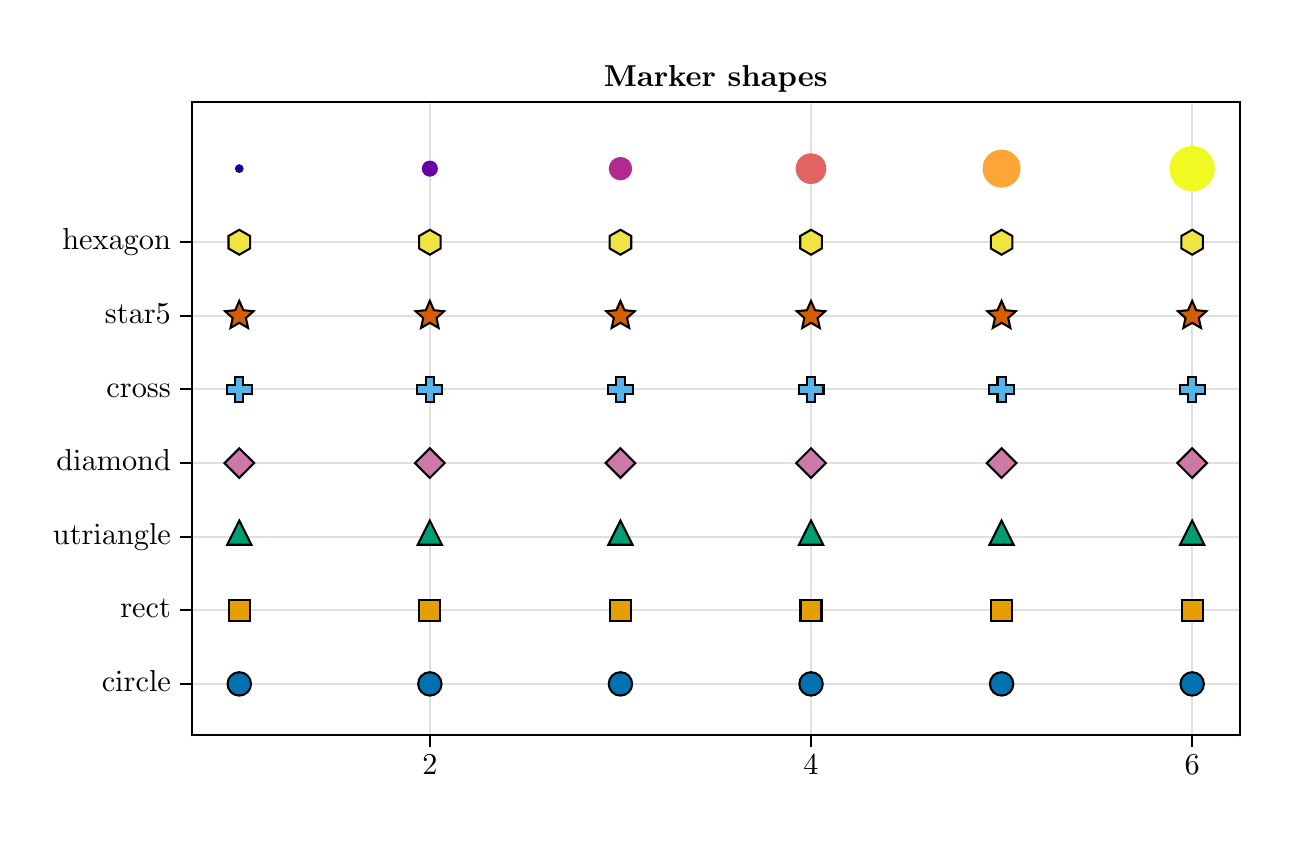
\begin{tikzpicture}[x=0.75pt, y=0.75pt, mknode/.style={inner sep=0pt, outer sep=0pt, execute at begin node={\vphantom{(}}, font=\fontsize{10.5}{12.6}\selectfont}, mkimg/.style={inner sep=0pt, outer sep=0pt}]
\definecolor{mkc1}{RGB}{0,114,178}
\definecolor{mkc2}{RGB}{230,159,0}
\definecolor{mkc3}{RGB}{0,158,115}
\definecolor{mkc4}{RGB}{204,121,167}
\definecolor{mkc5}{RGB}{86,180,233}
\definecolor{mkc6}{RGB}{213,94,0}
\definecolor{mkc7}{RGB}{240,228,66}
\definecolor{mkc8}{RGB}{13,8,135}
\definecolor{mkc9}{RGB}{106,0,168}
\definecolor{mkc10}{RGB}{177,42,144}
\definecolor{mkc11}{RGB}{225,100,98}
\definecolor{mkc12}{RGB}{252,166,54}
\definecolor{mkc13}{RGB}{240,249,33}
\path[use as bounding box] (0,0) rectangle (600,380);
\path[fill=white] (79,39) -- (584,39) -- (584,344) -- (79,344) -- cycle;
\draw[draw=black, line width=0.75pt, draw opacity=0.12]
  (193.77,39) -- (193.77,344)
  (377.41,39) -- (377.41,344)
  (561.05,39) -- (561.05,344);
\draw[draw=black, line width=0.75pt, draw opacity=0.12]
  (79,63.83) -- (584,63.83)
  (79,99.29) -- (584,99.29)
  (79,134.76) -- (584,134.76)
  (79,170.22) -- (584,170.22)
  (79,205.69) -- (584,205.69)
  (79,241.15) -- (584,241.15)
  (79,276.62) -- (584,276.62);
\node[mknode, anchor=north] at (193.77,31) {$2$};
\node[mknode, anchor=north] at (377.41,31) {$4$};
\node[mknode, anchor=north] at (561.05,31) {$6$};
\node[mknode, anchor=east] at (69,63.83) {circle};
\node[mknode, anchor=east] at (69,99.29) {rect};
\node[mknode, anchor=east] at (69,134.76) {utriangle};
\node[mknode, anchor=east] at (69,170.22) {diamond};
\node[mknode, anchor=east] at (69,205.69) {cross};
\node[mknode, anchor=east] at (69,241.15) {star5};
\node[mknode, anchor=east] at (69,276.62) {hexagon};
\node[mknode, anchor=south, font=\fontsize{10.5}{12.6}\selectfont\bfseries] at (331.5,348) {Marker shapes};
\begin{scope}
\clip (79,39) rectangle (584,344);
\path[fill=mkc1, draw=black, line width=0.75pt] (107.59,63.83) -- (107.59,63.83) .. controls (107.59,66.94) and (105.07,69.47) .. (101.95,69.47) .. controls (98.84,69.47) and (96.31,66.94) .. (96.31,63.83) .. controls (96.31,60.71) and (98.84,58.19) .. (101.95,58.19) .. controls (105.07,58.19) and (107.59,60.71) .. (107.59,63.83) -- cycle;
\path[fill=mkc1, draw=black, line width=0.75pt] (199.41,63.83) -- (199.41,63.83) .. controls (199.41,66.94) and (196.89,69.47) .. (193.77,69.47) .. controls (190.66,69.47) and (188.13,66.94) .. (188.13,63.83) .. controls (188.13,60.71) and (190.66,58.19) .. (193.77,58.19) .. controls (196.89,58.19) and (199.41,60.71) .. (199.41,63.83) -- cycle;
\path[fill=mkc1, draw=black, line width=0.75pt] (291.23,63.83) -- (291.23,63.83) .. controls (291.23,66.94) and (288.71,69.47) .. (285.59,69.47) .. controls (282.48,69.47) and (279.95,66.94) .. (279.95,63.83) .. controls (279.95,60.71) and (282.48,58.19) .. (285.59,58.19) .. controls (288.71,58.19) and (291.23,60.71) .. (291.23,63.83) -- cycle;
\path[fill=mkc1, draw=black, line width=0.75pt] (383.05,63.83) -- (383.05,63.83) .. controls (383.05,66.94) and (380.52,69.47) .. (377.41,69.47) .. controls (374.29,69.47) and (371.77,66.94) .. (371.77,63.83) .. controls (371.77,60.71) and (374.29,58.19) .. (377.41,58.19) .. controls (380.52,58.19) and (383.05,60.71) .. (383.05,63.83) -- cycle;
\path[fill=mkc1, draw=black, line width=0.75pt] (474.87,63.83) -- (474.87,63.83) .. controls (474.87,66.94) and (472.34,69.47) .. (469.23,69.47) .. controls (466.11,69.47) and (463.59,66.94) .. (463.59,63.83) .. controls (463.59,60.71) and (466.11,58.19) .. (469.23,58.19) .. controls (472.34,58.19) and (474.87,60.71) .. (474.87,63.83) -- cycle;
\path[fill=mkc1, draw=black, line width=0.75pt] (566.69,63.83) -- (566.69,63.83) .. controls (566.69,66.94) and (564.16,69.47) .. (561.05,69.47) .. controls (557.93,69.47) and (555.41,66.94) .. (555.41,63.83) .. controls (555.41,60.71) and (557.93,58.19) .. (561.05,58.19) .. controls (564.16,58.19) and (566.69,60.71) .. (566.69,63.83) -- cycle;
\path[fill=mkc2, draw=black, line width=0.75pt] (107.01,94.24) -- (107.01,104.34) -- (96.9,104.34) -- (96.9,94.24) -- cycle;
\path[fill=mkc2, draw=black, line width=0.75pt] (198.82,94.24) -- (198.82,104.34) -- (188.72,104.34) -- (188.72,94.24) -- cycle;
\path[fill=mkc2, draw=black, line width=0.75pt] (290.64,94.24) -- (290.64,104.34) -- (280.54,104.34) -- (280.54,94.24) -- cycle;
\path[fill=mkc2, draw=black, line width=0.75pt] (382.46,94.24) -- (382.46,104.34) -- (372.36,104.34) -- (372.36,94.24) -- cycle;
\path[fill=mkc2, draw=black, line width=0.75pt] (474.28,94.24) -- (474.28,104.34) -- (464.18,104.34) -- (464.18,94.24) -- cycle;
\path[fill=mkc2, draw=black, line width=0.75pt] (566.1,94.24) -- (566.1,104.34) -- (555.99,104.34) -- (555.99,94.24) -- cycle;
\path[fill=mkc3, draw=black, line width=0.75pt] (101.95,142.52) -- (96.13,130.88) -- (107.77,130.88) -- cycle;
\path[fill=mkc3, draw=black, line width=0.75pt] (193.77,142.52) -- (187.95,130.88) -- (199.59,130.88) -- cycle;
\path[fill=mkc3, draw=black, line width=0.75pt] (285.59,142.52) -- (279.77,130.88) -- (291.41,130.88) -- cycle;
\path[fill=mkc3, draw=black, line width=0.75pt] (377.41,142.52) -- (371.59,130.88) -- (383.23,130.88) -- cycle;
\path[fill=mkc3, draw=black, line width=0.75pt] (469.23,142.52) -- (463.41,130.88) -- (475.05,130.88) -- cycle;
\path[fill=mkc3, draw=black, line width=0.75pt] (561.05,142.52) -- (555.23,130.88) -- (566.87,130.88) -- cycle;
\path[fill=mkc4, draw=black, line width=0.75pt] (109.1,170.22) -- (101.95,177.36) -- (94.81,170.22) -- (101.95,163.08) -- cycle;
\path[fill=mkc4, draw=black, line width=0.75pt] (200.92,170.22) -- (193.77,177.36) -- (186.63,170.22) -- (193.77,163.08) -- cycle;
\path[fill=mkc4, draw=black, line width=0.75pt] (292.73,170.22) -- (285.59,177.36) -- (278.45,170.22) -- (285.59,163.08) -- cycle;
\path[fill=mkc4, draw=black, line width=0.75pt] (384.55,170.22) -- (377.41,177.36) -- (370.27,170.22) -- (377.41,163.08) -- cycle;
\path[fill=mkc4, draw=black, line width=0.75pt] (476.37,170.22) -- (469.23,177.36) -- (462.08,170.22) -- (469.23,163.08) -- cycle;
\path[fill=mkc4, draw=black, line width=0.75pt] (568.19,170.22) -- (561.05,177.36) -- (553.9,170.22) -- (561.05,163.08) -- cycle;
\path[fill=mkc5, draw=black, line width=0.75pt] (103.95,211.69) -- (103.95,207.68) -- (107.95,207.68) -- (107.95,203.69) -- (103.95,203.69) -- (103.95,199.69) -- (99.96,199.69) -- (99.96,203.69) -- (95.95,203.69) -- (95.95,207.68) -- (99.96,207.68) -- (99.96,211.69) -- cycle;
\path[fill=mkc5, draw=black, line width=0.75pt] (195.76,211.69) -- (195.76,207.68) -- (199.77,207.68) -- (199.77,203.69) -- (195.76,203.69) -- (195.76,199.69) -- (191.78,199.69) -- (191.78,203.69) -- (187.77,203.69) -- (187.77,207.68) -- (191.78,207.68) -- (191.78,211.69) -- cycle;
\path[fill=mkc5, draw=black, line width=0.75pt] (287.58,211.69) -- (287.58,207.68) -- (291.59,207.68) -- (291.59,203.69) -- (287.58,203.69) -- (287.58,199.69) -- (283.6,199.69) -- (283.6,203.69) -- (279.59,203.69) -- (279.59,207.68) -- (283.6,207.68) -- (283.6,211.69) -- cycle;
\path[fill=mkc5, draw=black, line width=0.75pt] (379.4,211.69) -- (379.4,207.68) -- (383.41,207.68) -- (383.41,203.69) -- (379.4,203.69) -- (379.4,199.69) -- (375.42,199.69) -- (375.42,203.69) -- (371.41,203.69) -- (371.41,207.68) -- (375.42,207.68) -- (375.42,211.69) -- cycle;
\path[fill=mkc5, draw=black, line width=0.75pt] (471.22,211.69) -- (471.22,207.68) -- (475.23,207.68) -- (475.23,203.69) -- (471.22,203.69) -- (471.22,199.69) -- (467.24,199.69) -- (467.24,203.69) -- (463.23,203.69) -- (463.23,207.68) -- (467.24,207.68) -- (467.24,211.69) -- cycle;
\path[fill=mkc5, draw=black, line width=0.75pt] (563.04,211.69) -- (563.04,207.68) -- (567.05,207.68) -- (567.05,203.69) -- (563.04,203.69) -- (563.04,199.69) -- (559.05,199.69) -- (559.05,203.69) -- (555.05,203.69) -- (555.05,207.68) -- (559.05,207.68) -- (559.05,211.69) -- cycle;
\path[fill=mkc6, draw=black, line width=0.75pt] (101.95,248.35) -- (99.98,243.87) -- (95.11,243.38) -- (98.76,240.11) -- (97.72,235.33) -- (101.95,237.79) -- (106.19,235.33) -- (105.15,240.11) -- (108.8,243.38) -- (103.93,243.87) -- cycle;
\path[fill=mkc6, draw=black, line width=0.75pt] (193.77,248.35) -- (191.8,243.87) -- (186.93,243.38) -- (190.58,240.11) -- (189.54,235.33) -- (193.77,237.79) -- (198,235.33) -- (196.97,240.11) -- (200.62,243.38) -- (195.75,243.87) -- cycle;
\path[fill=mkc6, draw=black, line width=0.75pt] (285.59,248.35) -- (283.62,243.87) -- (278.74,243.38) -- (282.4,240.11) -- (281.36,235.33) -- (285.59,237.79) -- (289.82,235.33) -- (288.79,240.11) -- (292.44,243.38) -- (287.57,243.87) -- cycle;
\path[fill=mkc6, draw=black, line width=0.75pt] (377.41,248.35) -- (375.43,243.87) -- (370.56,243.38) -- (374.21,240.11) -- (373.18,235.33) -- (377.41,237.79) -- (381.64,235.33) -- (380.6,240.11) -- (384.26,243.38) -- (379.38,243.87) -- cycle;
\path[fill=mkc6, draw=black, line width=0.75pt] (469.23,248.35) -- (467.25,243.87) -- (462.38,243.38) -- (466.03,240.11) -- (465,235.33) -- (469.23,237.79) -- (473.46,235.33) -- (472.42,240.11) -- (476.07,243.38) -- (471.2,243.87) -- cycle;
\path[fill=mkc6, draw=black, line width=0.75pt] (561.05,248.35) -- (559.07,243.87) -- (554.2,243.38) -- (557.85,240.11) -- (556.81,235.33) -- (561.05,237.79) -- (565.28,235.33) -- (564.24,240.11) -- (567.89,243.38) -- (563.02,243.87) -- cycle;
\path[fill=mkc7, draw=black, line width=0.75pt] (101.95,282.62) -- (96.76,279.62) -- (96.76,273.62) -- (101.95,270.62) -- (107.15,273.62) -- (107.15,279.62) -- cycle;
\path[fill=mkc7, draw=black, line width=0.75pt] (193.77,282.62) -- (188.58,279.62) -- (188.58,273.62) -- (193.77,270.62) -- (198.97,273.62) -- (198.97,279.62) -- cycle;
\path[fill=mkc7, draw=black, line width=0.75pt] (285.59,282.62) -- (280.39,279.62) -- (280.39,273.62) -- (285.59,270.62) -- (290.79,273.62) -- (290.79,279.62) -- cycle;
\path[fill=mkc7, draw=black, line width=0.75pt] (377.41,282.62) -- (372.21,279.62) -- (372.21,273.62) -- (377.41,270.62) -- (382.61,273.62) -- (382.61,279.62) -- cycle;
\path[fill=mkc7, draw=black, line width=0.75pt] (469.23,282.62) -- (464.03,279.62) -- (464.03,273.62) -- (469.23,270.62) -- (474.42,273.62) -- (474.42,279.62) -- cycle;
\path[fill=mkc7, draw=black, line width=0.75pt] (561.05,282.62) -- (555.85,279.62) -- (555.85,273.62) -- (561.05,270.62) -- (566.24,273.62) -- (566.24,279.62) -- cycle;
\path[fill=mkc8] (104.07,312.08) -- (104.07,312.08) .. controls (104.07,313.25) and (103.12,314.2) .. (101.95,314.2) .. controls (100.79,314.2) and (99.84,313.25) .. (99.84,312.08) .. controls (99.84,310.91) and (100.79,309.97) .. (101.95,309.97) .. controls (103.12,309.97) and (104.07,310.91) .. (104.07,312.08) -- cycle;
\path[fill=mkc9] (197.65,312.08) -- (197.65,312.08) .. controls (197.65,314.22) and (195.91,315.96) .. (193.77,315.96) .. controls (191.63,315.96) and (189.9,314.22) .. (189.9,312.08) .. controls (189.9,309.94) and (191.63,308.2) .. (193.77,308.2) .. controls (195.91,308.2) and (197.65,309.94) .. (197.65,312.08) -- cycle;
\path[fill=mkc10] (291.23,312.08) -- (291.23,312.08) .. controls (291.23,315.2) and (288.71,317.72) .. (285.59,317.72) .. controls (282.48,317.72) and (279.95,315.2) .. (279.95,312.08) .. controls (279.95,308.97) and (282.48,306.44) .. (285.59,306.44) .. controls (288.71,306.44) and (291.23,308.97) .. (291.23,312.08) -- cycle;
\path[fill=mkc11] (384.81,312.08) -- (384.81,312.08) .. controls (384.81,316.17) and (381.5,319.48) .. (377.41,319.48) .. controls (373.32,319.48) and (370.01,316.17) .. (370.01,312.08) .. controls (370.01,307.99) and (373.32,304.68) .. (377.41,304.68) .. controls (381.5,304.68) and (384.81,307.99) .. (384.81,312.08) -- cycle;
\path[fill=mkc12] (478.39,312.08) -- (478.39,312.08) .. controls (478.39,317.14) and (474.29,321.25) .. (469.23,321.25) .. controls (464.17,321.25) and (460.06,317.14) .. (460.06,312.08) .. controls (460.06,307.02) and (464.17,302.92) .. (469.23,302.92) .. controls (474.29,302.92) and (478.39,307.02) .. (478.39,312.08) -- cycle;
\path[fill=mkc13] (571.97,312.08) -- (571.97,312.08) .. controls (571.97,318.12) and (567.08,323.01) .. (561.05,323.01) .. controls (555.01,323.01) and (550.12,318.12) .. (550.12,312.08) .. controls (550.12,306.05) and (555.01,301.15) .. (561.05,301.15) .. controls (567.08,301.15) and (571.97,306.05) .. (571.97,312.08) -- cycle;
\end{scope}
\draw[draw=black, line width=0.75pt]
  (193.77,38.5) -- (193.77,33.5)
  (377.41,38.5) -- (377.41,33.5)
  (561.05,38.5) -- (561.05,33.5);
\draw[draw=black, line width=0.75pt]
  (78.5,63.83) -- (73.5,63.83)
  (78.5,99.29) -- (73.5,99.29)
  (78.5,134.76) -- (73.5,134.76)
  (78.5,170.22) -- (73.5,170.22)
  (78.5,205.69) -- (73.5,205.69)
  (78.5,241.15) -- (73.5,241.15)
  (78.5,276.62) -- (73.5,276.62);
\draw[draw=black, line width=0.75pt]
  (78.5,39) -- (584.5,39);
\draw[draw=black, line width=0.75pt]
  (79,38.5) -- (79,344.5);
\draw[draw=black, line width=0.75pt]
  (78.5,344) -- (584.5,344);
\draw[draw=black, line width=0.75pt]
  (584,38.5) -- (584,344.5);
\end{tikzpicture}
